%%%%%%%%%%%%%%%%%%%%%%%%%%%%%%%%%%%%%%%%%%%%%%
%                insertmeeting
% 1) Title (something creative & funny?)
% 2) Date (MM/DD/YYYY)
% 3) Location (ex. Hagerty High School)
% 4) People/Committees Present 
% 5) Picture 
% 6) Start Time & Stop Time (ex. 12:30AM to 4:30PM)
%%%%%%%%%%%%%%%%%%%%%%%%%%%%%%%%%%%%%%%%%%%%%%
\insertmeeting 
	{Drivetrain Programming} 
	{09/14/21}
	{Hagerty High School}
	{Annika, Anouska, Clayton, Falon, James, Jensen, Nathan, Ritam, Rose, Samantha, Lilly}
	{Images/RobotPics/robot.jpg}
	{2:30 - 4:30}
	
\subsection*{Software}
\noindent\hfil\rule{\textwidth}{.4pt}\hfil
\subsubsection*{Goals}
\begin{itemize}
    \item Continue with work on the tele op for new Mecanum Drive 

\end{itemize} 

\noindent\hfil\rule{\textwidth}{.4pt}\hfil

\subsubsection*{Accomplishments}
During this meeting, we continued to debug the TRC code and work on the tele-op for our Mecanum Drive. We were having issues as the robot was going in an arc and decided to incorporate encoders within Tele-Op. We decided to use RUN WITH ENCODER (line 50 on picture shown below) which uses the Hardware PID to be able to maintain a specific velocity. This is important because the motors themselves could be going at different speeds, a difficulty we discovered at the previous meeting after recording the encoder ticks. We plan to test our new revison at the next meeting. Next, we plan to continue working on tele op and fixing the Arc problem when Strafing

\begin{figure}[htp]
\centering
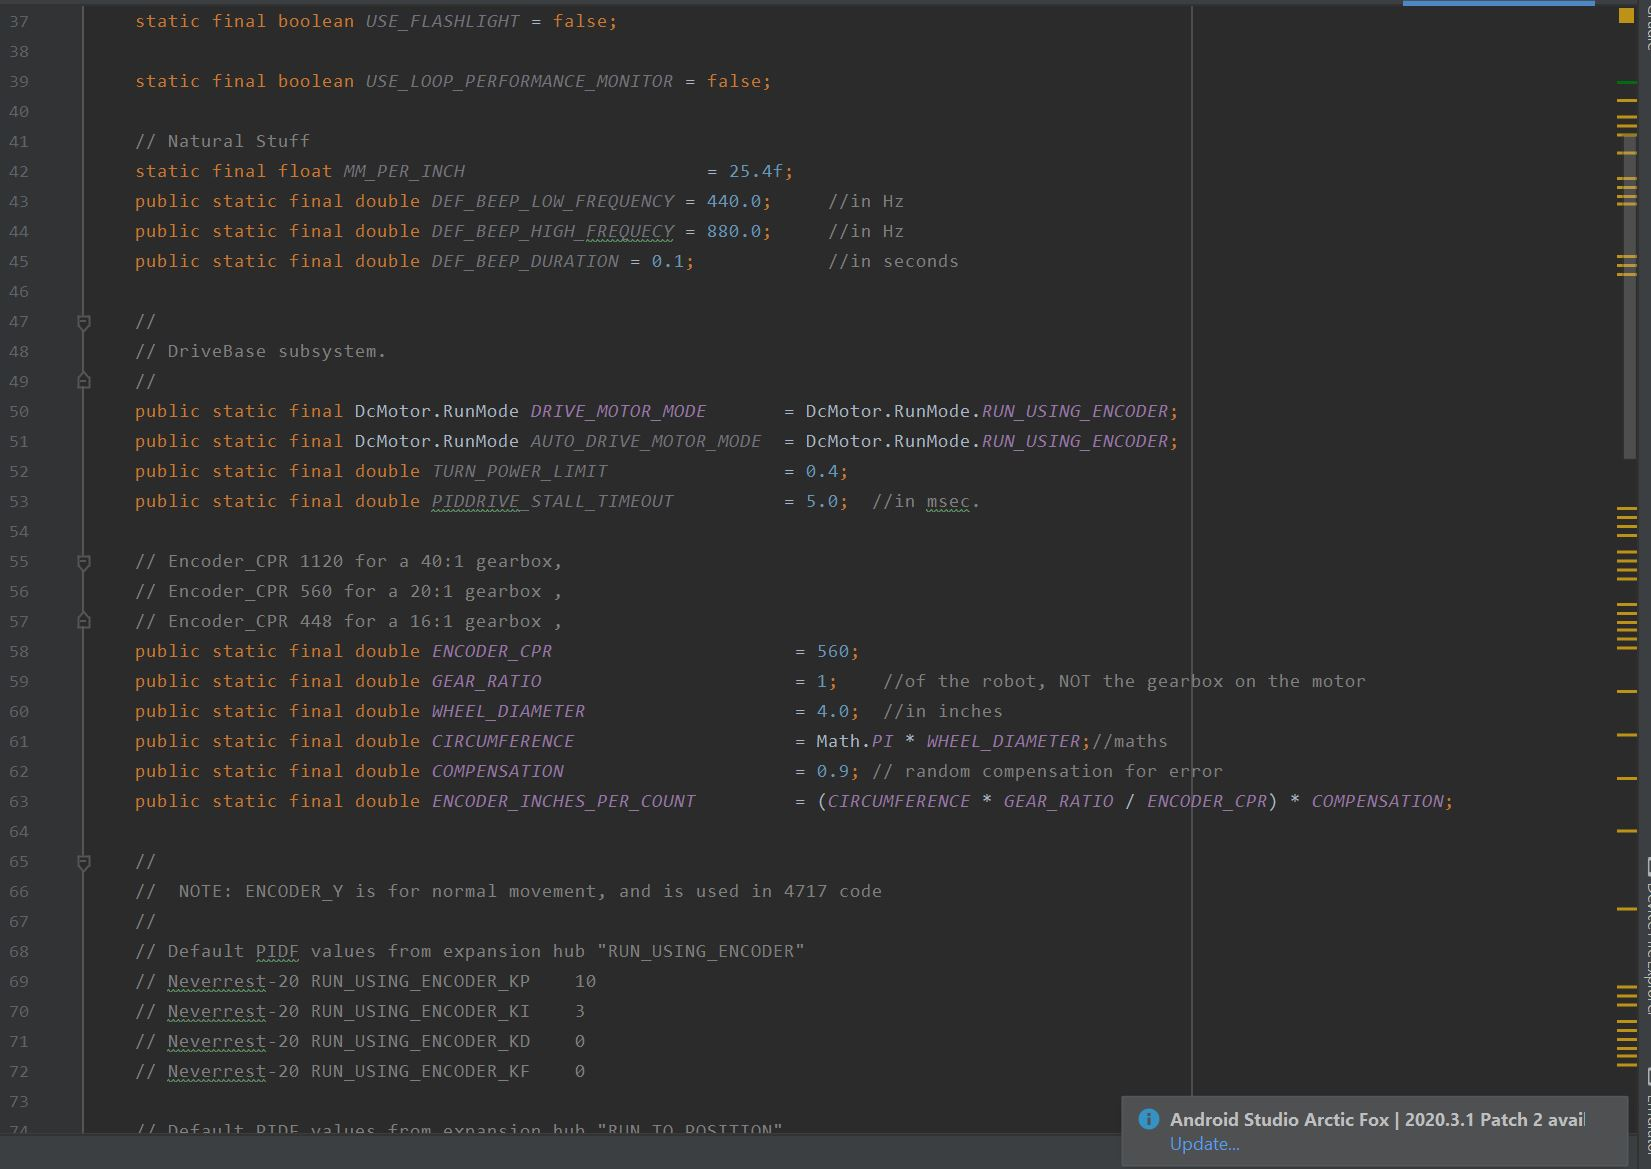
\includegraphics[width=0.9\textwidth, angle=0]{Meetings/September/09-14-21/09-14-21 1.JPG}
\caption{Our new Robot constants for use in later drivetrain testing.}
\label{fig:pic1}
\end{figure}

